%% LaTeX Beamer presentation template (requires beamer package)
%% see http://bitbucket.org/rivanvx/beamer/wiki/Home
%% idea contributed by H. Turgut Uyar
%% template based on a template by Till Tantau
%% this template is still evolving - it might differ in future releases!

\documentclass{beamer}

\mode<presentation>
{
\usetheme{Warsaw}

\setbeamercovered{transparent}
}

\usepackage[english]{babel}
\usepackage[latin1]{inputenc}

% font definitions, try \usepackage{ae} instead of the following
% three lines if you don't like this look
\usepackage{mathptmx}
\usepackage[scaled=.90]{helvet}
\usepackage{courier}


\usepackage[T1]{fontenc}


\title{Persistence in practice}

% \subtitle{M.Sc. Eng. defense}

\author{Sune~Keller}
\date{December 14, 2012}
% This is only inserted into the PDF information catalog. Can be left
% out.
\subject{M.Sc. Eng. defense}

% Delete this, if you do not want the table of contents to pop up at
% the beginning of each subsection:
% \AtBeginSubsection[]
% {
% \begin{frame}<beamer>
% \frametitle{Outline}
% \tableofcontents[currentsection,currentsubsection]
% \end{frame}
% }

% If you wish to uncover everything in a step-wise fashion, uncomment
% the following command:

%\beamerdefaultoverlayspecification{<+->}

\begin{document}

\begin{frame}
\titlepage
\end{frame}

\begin{frame}
\frametitle{Outline}
\tableofcontents[pausesections]
% You might wish to add the option [pausesections]
\end{frame}


\section{Introduction}

\begin{frame}
\frametitle{Partially Persistent Data Structures}
\begin{itemize}
  \item All versions available for access
  \pause
  \item New versions can be appended onto the most recent
  \pause
  \item All DS operations should be supported
  \pause
  \begin{itemize}
    \item Linked list: \textsc{head}, \textsc{size} at all versions,\newline\hphantom{Linked list: }\textsc{data} fields, \textsc{next} pointers from nodes
  \end{itemize}
  \pause
  \item Mentioned as ``rollback databases'' in \cite{10.1109/AFIPS.1987.11}
\end{itemize}
\end{frame}

\section{Method}

\subsection{Node Copying}

\begin{frame}
\frametitle{Node Copying}
\begin{itemize}
  \item Any bounded in-degree DS \cite{Driscoll198986}
  \item Expands node structure
  \begin{itemize}
    \item Modifications
    \item Back pointers
  \end{itemize}
  \item Adds auxillary structure for maintaining entry points (e.g. head)
\end{itemize}
\pause
\begin{figure}
\center
\only<1>{\vphantom{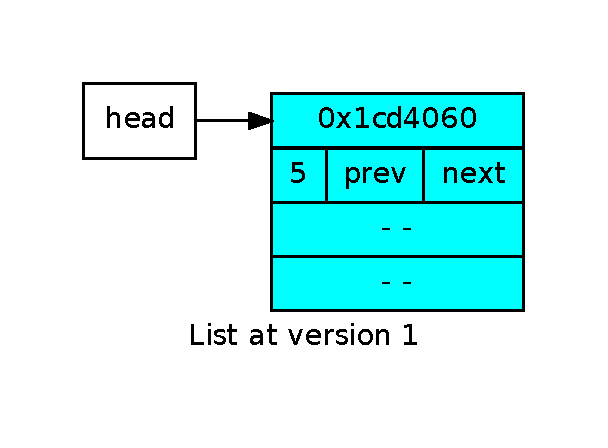
\includegraphics[height=0.55\textheight]{figures/v1.pdf}}}
\only<2>{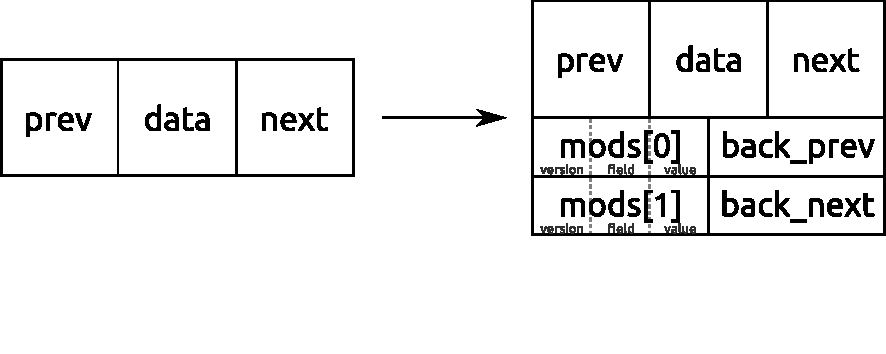
\includegraphics[height=0.55\textheight]{figures/node-copying-example.pdf}}
\only<3>{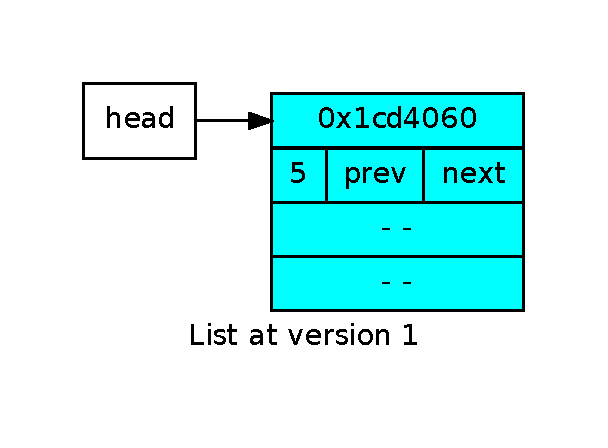
\includegraphics[height=0.55\textheight]{figures/v1.pdf}}
\only<4>{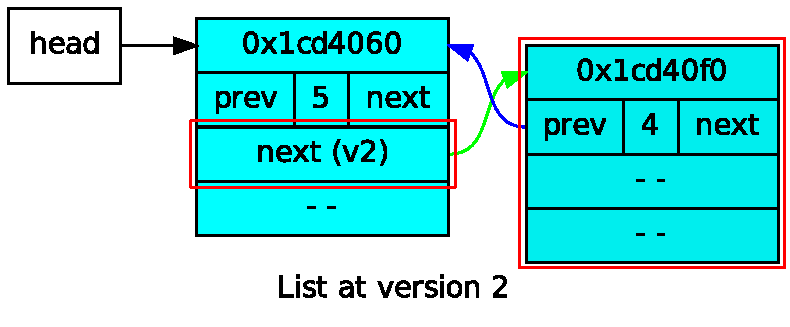
\includegraphics[height=0.55\textheight]{figures/v2.pdf}}
\only<5>{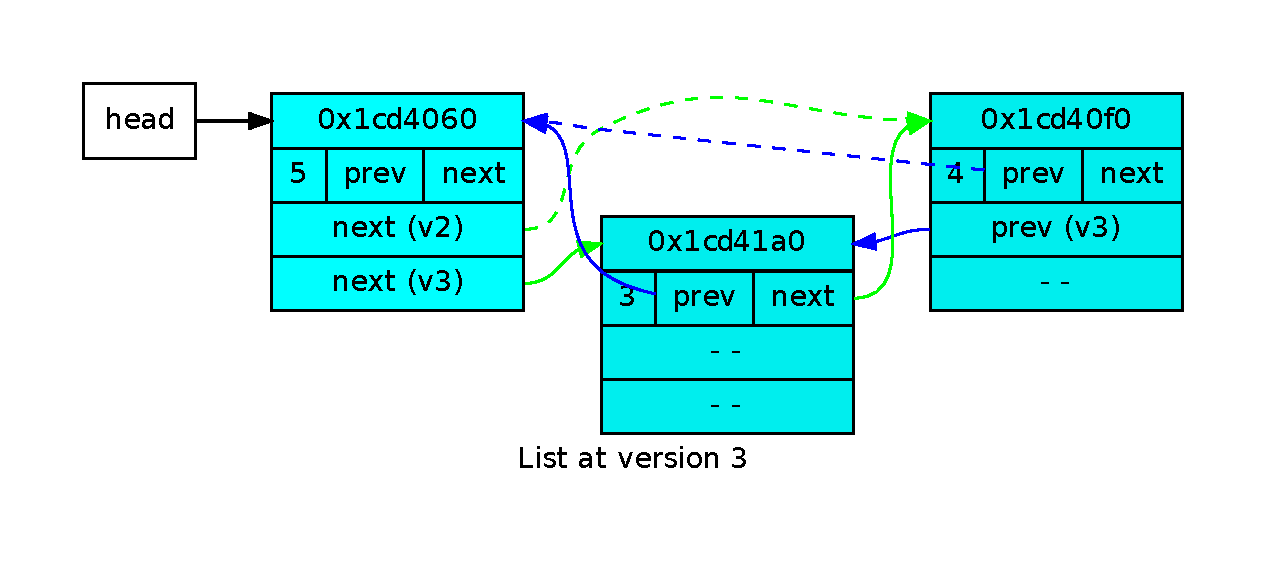
\includegraphics[height=0.55\textheight]{figures/v3.pdf}}
\only<6>{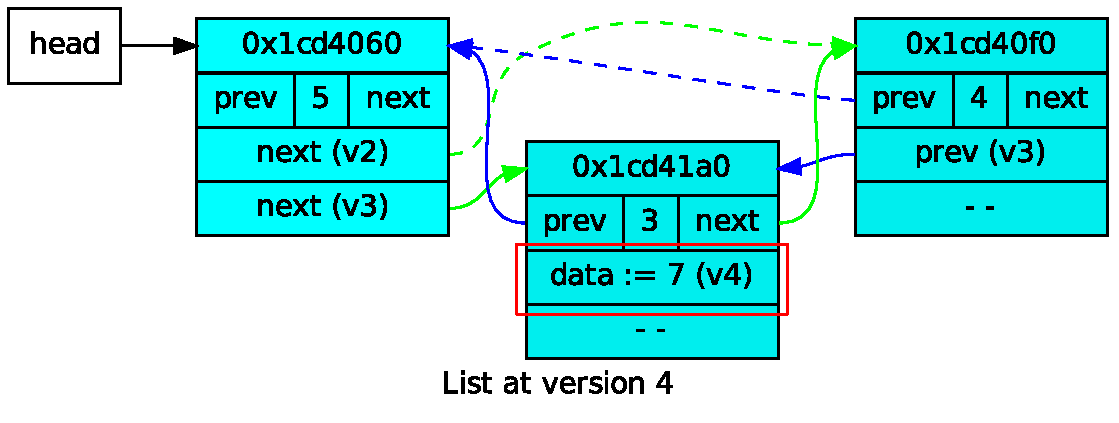
\includegraphics[height=0.55\textheight]{figures/v4.pdf}}
\only<7>{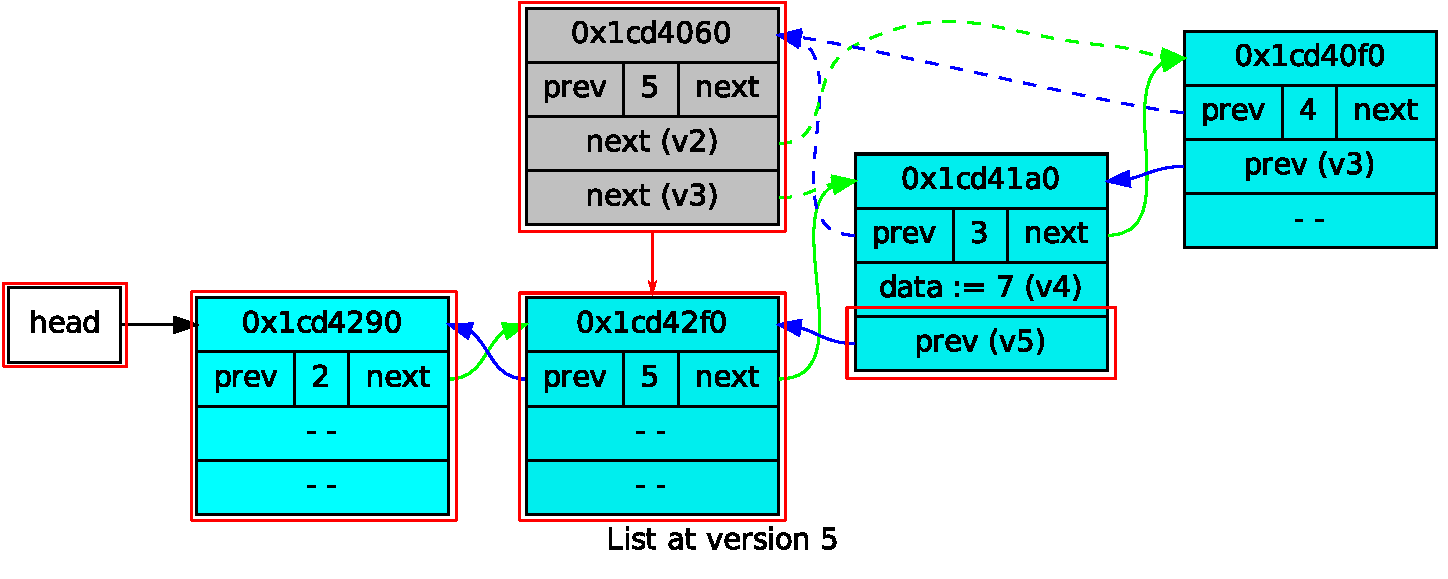
\includegraphics[height=0.55\textheight]{figures/v5.pdf}}
\only<8>{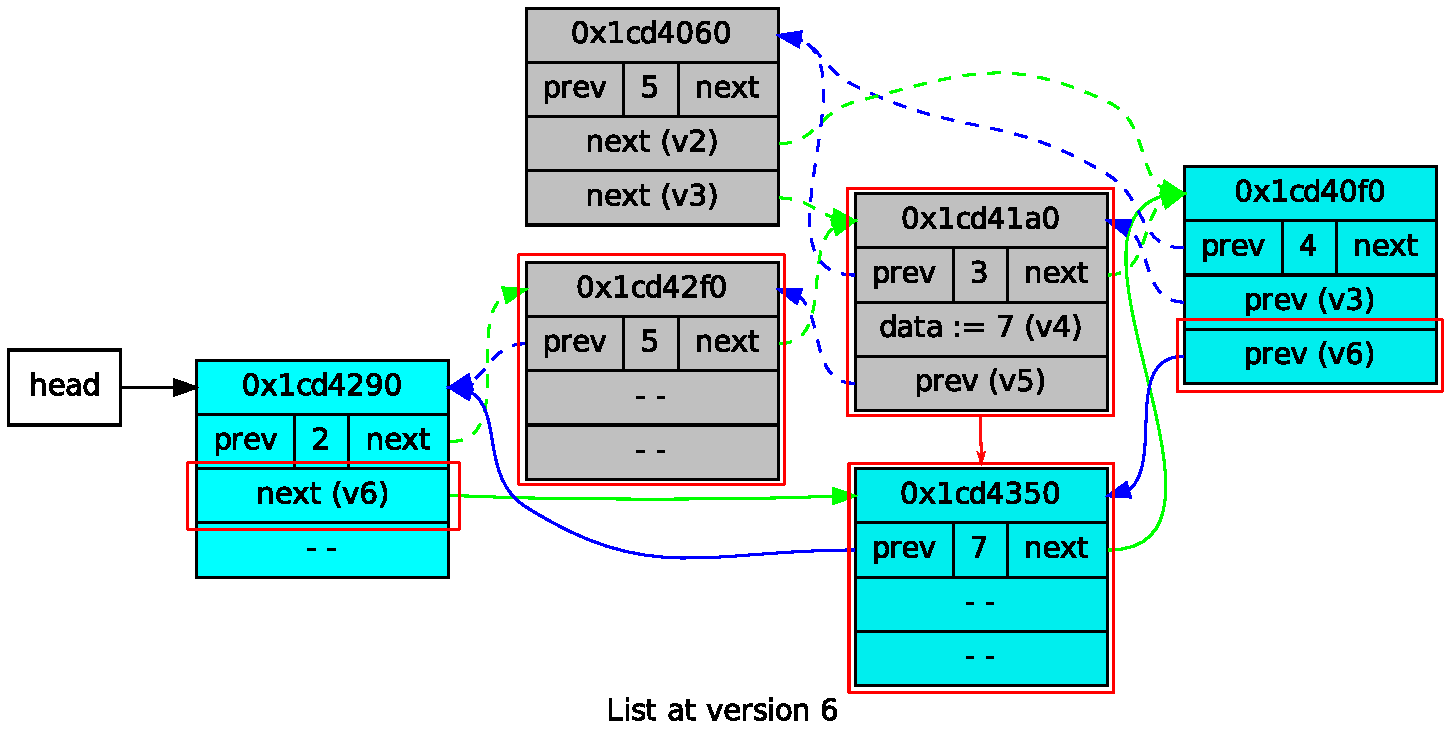
\includegraphics[height=0.55\textheight]{figures/v6.pdf}}
\only<9>{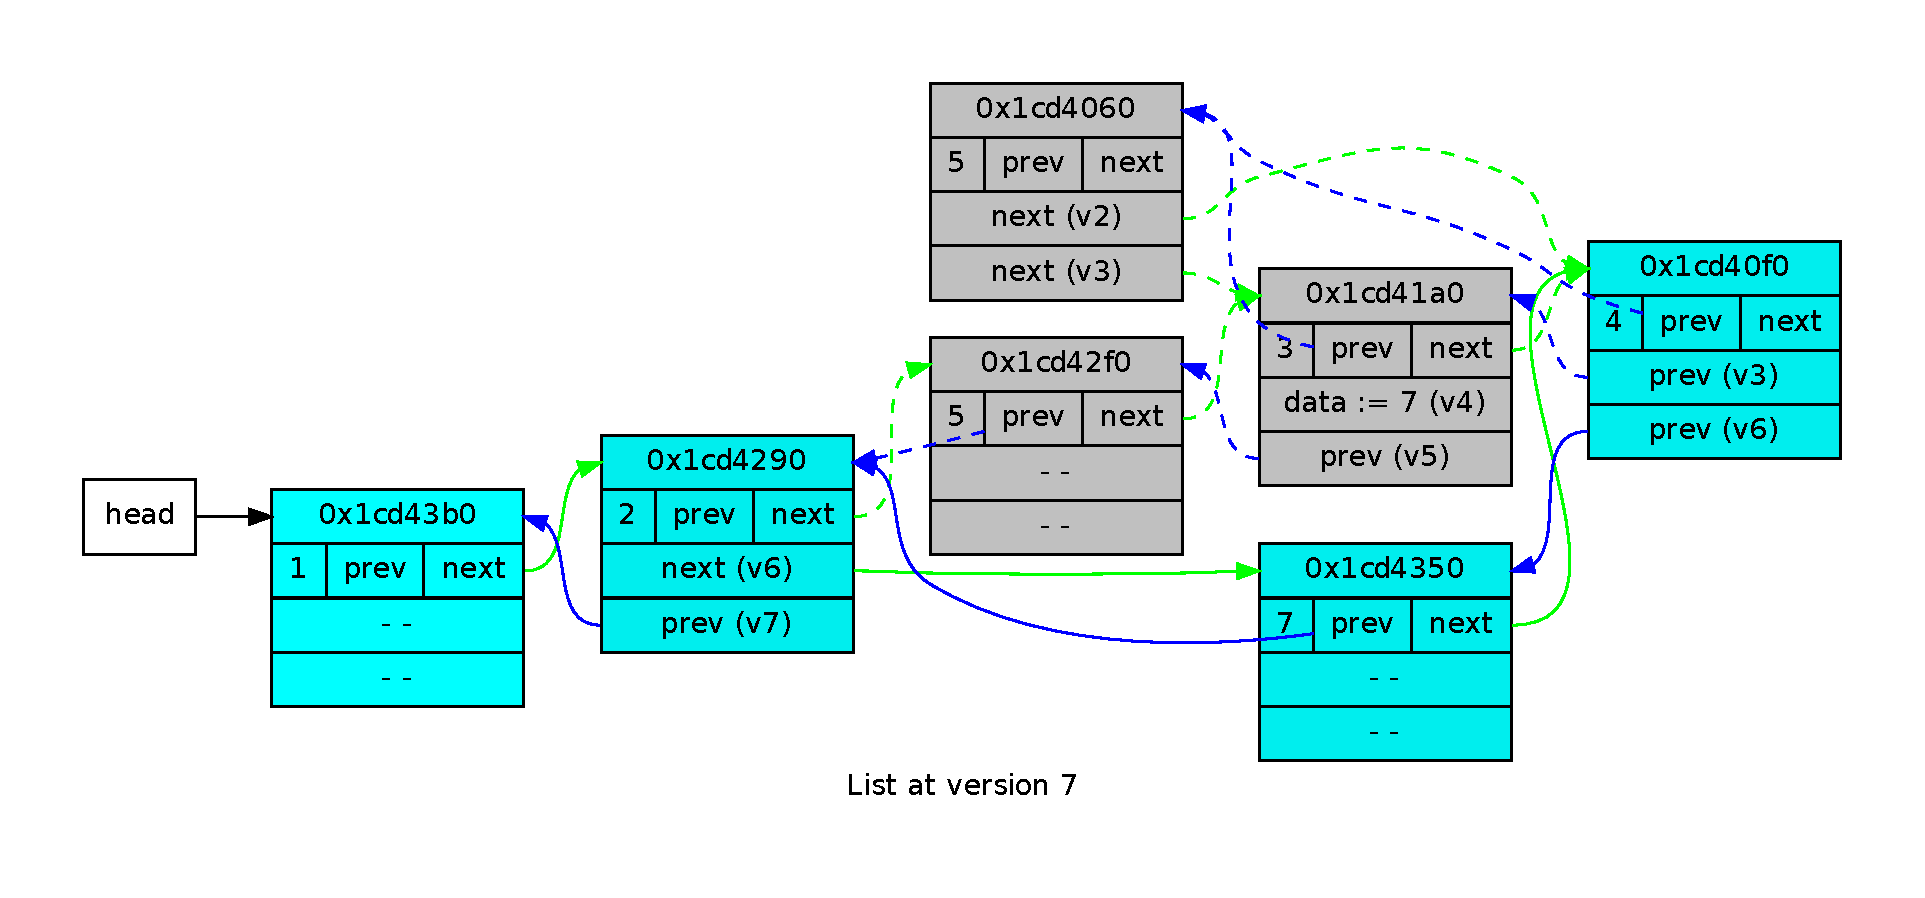
\includegraphics[height=0.55\textheight]{figures/v7.pdf}}
\end{figure}
\end{frame}

\subsection{Rollback}
\begin{frame}
\frametitle{Rollback}
\begin{itemize}
  \item Hybrid of two na\"ive approaches ``log'', ``copy'' defined in \cite{Tsotras1995237}
  \begin{itemize}
    \item The paper deals with several, more advanced DS, including a hybrid
  \end{itemize}
  \pause
  \item The ``log'' approach stores all operations with inversion info
  \pause
  \item The ``copy'' approach stores full copy of every version
  \pause
  \item Rollback stores log for every operation, full copy of every $d$ versions
\end{itemize}
\end{frame}

\section{Empirical Analysis}

\begin{frame}
\frametitle{Empirical Analysis}
\begin{itemize}
  \item Four operation types:
  \begin{itemize}

    \item \textsc{insert}$(i, d)$, \textsc{modify}$(i, d)$, \textsc{remove}$(i)$
    \& \textsc{access}$(v, i)$

  \end{itemize}
  \item Two usage scenarios:
  \begin{itemize}

    \item Sequential: $\frac{1}{4}c$ of each operation in above order

    \item Random: $c$ operations, $p=\frac{1}{4}$ for each type
    \begin{itemize}
      \item ${}\implies p_{insert}=p_{remove}$, expected mean change in list size is 0
    \end{itemize}
  \end{itemize}

\end{itemize}
\end{frame}

\subsection{Implementation overview}

\begin{frame}
\frametitle{Implementation overview}
\begin{itemize}
  \item Three implementations:

  \begin{itemize}
    \item Node Copying
    \item Rollback -- Blackbox variant
    \item Rollback -- Eliminate-Reorder variant
  \end{itemize}
\end{itemize}
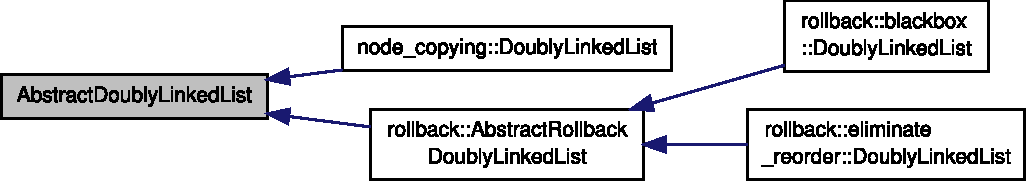
\includegraphics[width=\textwidth]{figures/classAbstractDoublyLinkedList__inherit__graph.pdf}
\end{frame}

\subsection{Experiments}


\begin{frame}
\frametitle{Experiments}
\begin{itemize}

  \item Duration measured separately for each operation type
  \begin{itemize}
    \item Actual count also recorded in Random scenario
  \end{itemize}

  \item 10 different operation counts, exponentially spaced in the range between
  1000 and 2000000 (both inclusive)

  \begin{itemize}

    \item Only the first 7 counts in Sequential usage scenario

  \end{itemize}

  \item 10 runs with each count, graphs show average durations and 95\%
  confidence intervals

  \begin{itemize}

    \item Note: Same seed passed to \texttt{srand()} with every experiment to
    produce comparable sequence orders in Random usage scenario

  \end{itemize}

  \item Memory usage estimates and duration measurements conducted independently
  --- we'll get to that later

\end{itemize}
\end{frame}

\subsection{Results}

\begin{frame}
\frametitle{Results: \textsc{insert} operations}
\begin{columns}[t]
  \begin{column}{0.55\textwidth}

      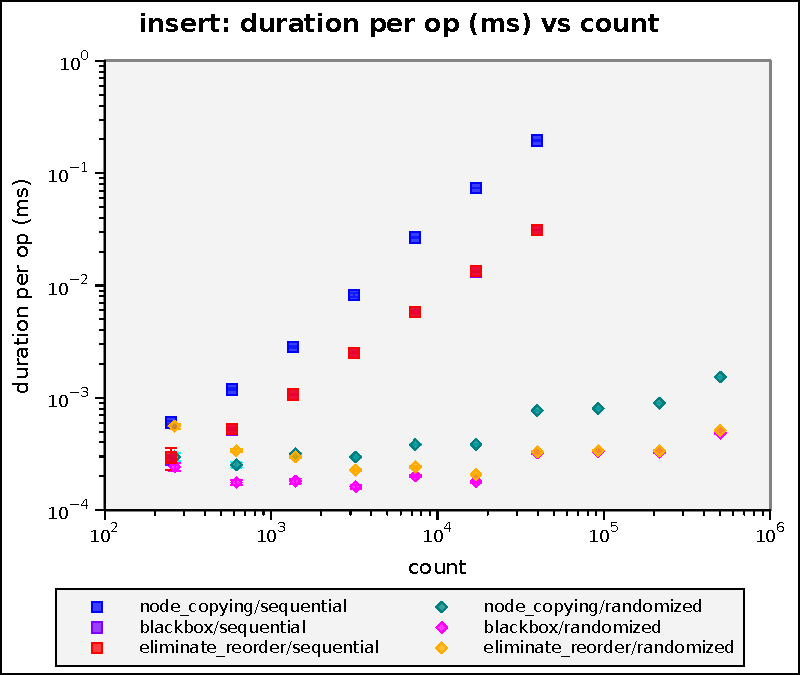
\includegraphics[height=0.65\textheight]{figures/graphs/insert-duration-per-op-vs-count.pdf}
      \newline Duration per \textsc{insert} operation in milliseconds\vphantom{ --- only head node}
  \end{column}

  \begin{column}{0.50\textwidth}
    \begin{itemize}

      \item Node Copying is slower at \textsc{insert} operations compared to either
      Rollback implementation, regardless of usage scenario

      \item Eliminate-Reorder is not faster than Blackbox at \textsc{insert}
      operations

    \end{itemize}
  \end{column}
\end{columns}
\end{frame}

\begin{frame}
\frametitle{Results: \textsc{access} operations}
\begin{columns}[t]
  \begin{column}{0.55\textwidth}

    \only<1>{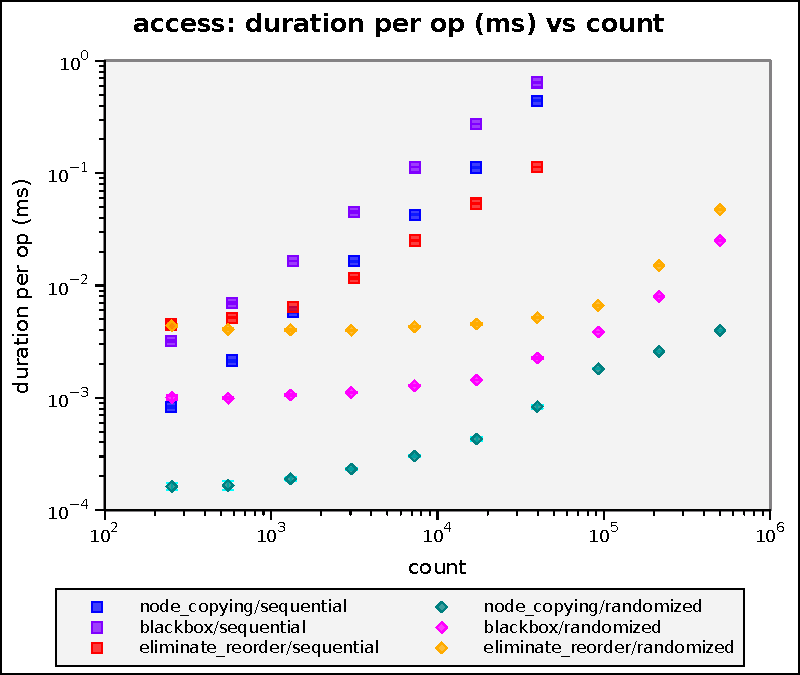
\includegraphics[height=0.65\textheight]{figures/graphs/access-duration-per-op-vs-count.pdf}}
    \only<2>{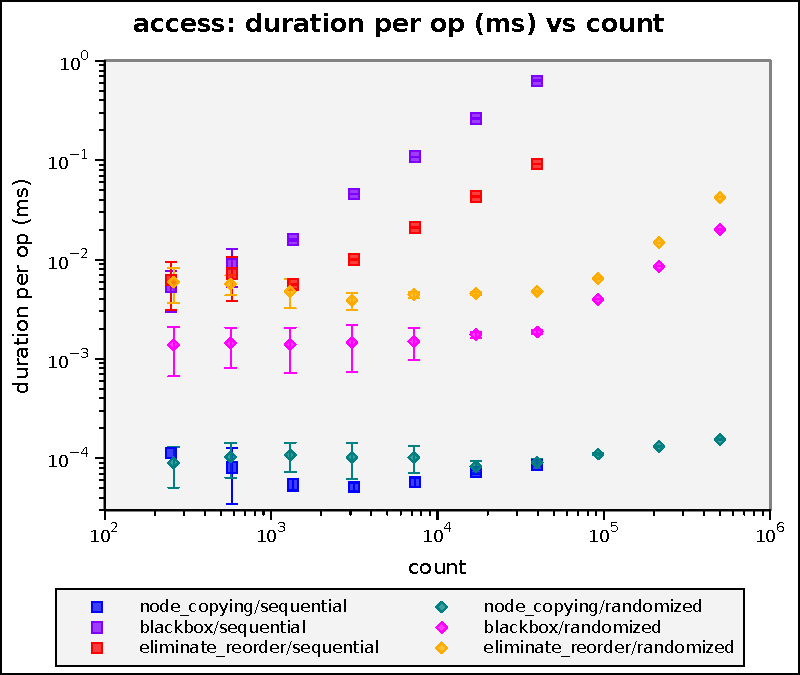
\includegraphics[height=0.65\textheight]{figures/graphs/access-duration-per-op-vs-count-head-only.pdf}}
    \newline \only<1>{Duration per \textsc{acccess} operation in milliseconds\vphantom{ --- only head node}}
    \only<2>{Duration per \textsc{acccess} operation in milliseconds --- only head node}
  \end{column}

  \begin{column}{0.50\textwidth}
    \begin{itemize}

      \item Node Copying is \textit{considerably} faster at \textsc{access}
      operations in the Random scenario, but in the Sequential scenario it is
      overtaken by Eliminate-Reorder

      \begin{itemize}
        \item The cost in memory usage is great, we'll get to that soon
      \end{itemize}

    \end{itemize}
  \end{column}
\end{columns}
\end{frame}

\begin{frame}
\frametitle{Memory usage estimates}
\begin{columns}[t]
  \begin{column}{0.55\textwidth}

    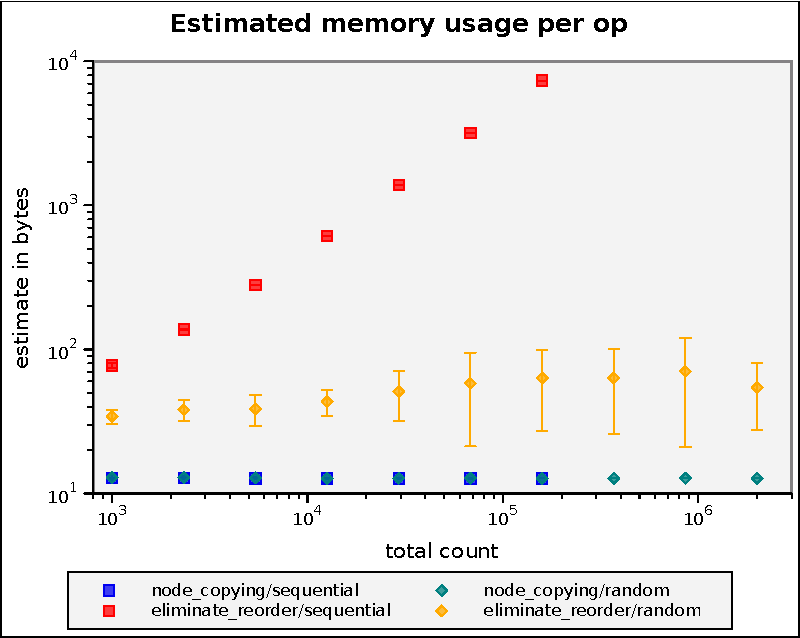
\includegraphics[height=0.65\textheight]{figures/graphs/space-results-per-op.pdf}
    \newline Estimated memory usage per operation in bytes
  \end{column}

  \begin{column}{0.50\textwidth}

    \begin{itemize}

      \item In the Sequential usage scenario, Rollback uses significantly more
      memory than Node Copying, and more so as \texttt{count} increases

      \item In the Random scenario, the benefit of Node Copying is still
      significant, but also considerably smaller.

    \end{itemize}

  \end{column}
\end{columns}
\end{frame}

\section*{Summary}

\begin{frame}
\frametitle<presentation>{Summary}

\begin{itemize}

  \item An optimized Rollback implementation may be up to half an order of
  magnitude faster at insertions than Node Copying, and at access in sequential
  scenarios with large enough data sets, but it falls short in the randomized
  scenario and in terms of memory usage.

\end{itemize}

\pause

% The following outlook is optional.
\vskip0pt plus.5fill
\begin{itemize}
  \item Future work:
  \begin{itemize}

    \item More advanced data structures

    \begin{itemize}

      \item BBSTs, RB trees, Binary heaps, 2-3-4 trees

    \end{itemize}

\pause
    \item More usage scenarios

    \begin{itemize}

      \item Front-to-back version access, algorithms (planar point location),
      functional use of DS (e.g. iterative depth-first algorithms on large data
      sets), intentionally worst-case scenarios, temporal databases, offline
      interval queries

    \end{itemize}

\pause
    \item Caching and other I/O optimizations (e.g. of Node Copying navigation),
    compression of full copies

  \end{itemize}
\end{itemize}
\end{frame}

\bgroup
\setbeamercolor{background canvas}{bg=white}
\begin{frame}[plain]{}
\center
\Huge
Questions?
\end{frame}
\egroup

\begin{frame}<beamer:0>
\frametitle{References}
\bibliographystyle{alpha}
\bibliography{References}
\end{frame}

\end{document}
